% how-to guide: https://www.sharelatex.com/blog/2013/08/13/beamer-series-pt1.html

\documentclass{beamer}
\usetheme{Warsaw}
\usepackage[utf8]{inputenc}
\usepackage[french]{babel}
\usepackage{graphicx}
\usepackage{tikz}

\title{Correcteur de posture assise à base d'Arduino}
\subtitle{\small DI 6}
\author[KOKKONIS Dimitrios \\\and LOCHE Jérémy]{\small {\small \texttt{Auteurs}}\\ KOKKONIS Dimitrios \\\and LOCHE Jérémy\\
\vspace{5px}
{\small \texttt{Encadrant}}\\ BEAUFILS Sébastien}
\institute{\textsc{École Polytechnique de l'Université de Tours}}
\date{11 mai 2017}

% new environments
\newenvironment{figim}[2]{%
	\begin{figure}[htbp]
	\caption{#1}
	\label{#2}
	\begin{center}
}{%
	\end{center}
	\end{figure}
}

\begin{document}

\begin{frame}
\vspace{0.1cm}

\includegraphics[height=1cm]{images/Logo_PeiP_v2009_RGB_3cm_300dpi.jpg}

\includegraphics[height=1cm]{images/logo_Polytech_Tours_RVB_3cm_300dpi.jpg}
\hfill

\includegraphics[height=1cm]{images/logo_UFR_4cm_300dpi.jpg}
\titlepage
\end{frame}

\begin{frame}
\frametitle{Plan}
\tableofcontents
\end{frame}

\section*{Introduction}
\begin{frame}
\begin{block}{Introduction}
\begin{itemize}
\pause
\item Objectif :
\pause
\begin{itemize}
\item Créer un correcteur de posture assise
\pause
\item Communiquer un résultat
\end{itemize}
\pause
\item Solution apportée :
\begin{itemize}
\pause
\item Création d'un système embarqué 
\end{itemize}
\end{itemize}
\end{block}
\end{frame}

\begin{frame}
\begin{block}{Plan du système :}
\pause
\begin{itemize}
\item 4 cellules de charge dont la résistance varie lorsqu'on applique une force sur eux
\pause
\item 4 ponts Wheatstone (construits à partir des cellules de charge) qui permettent de mésurer une tension
\pause
\item 4 amplificateurs qui amplifient le signal fourni par les cellules de charge
\pause
\item un Arduino Uno, qui récupère les données fournies par les amplificateurs, les traite, et les envoie à l'application
\pause
\item une application (PC ou Android), qui reçoit les données de l'Arduino (par Bluetooth ou par USB) et permet de visualiser la posture à partir de ces données
\end{itemize}
\end{block}
\end{frame}

\section{Les cellules de charge}
\begin{frame}
\begin{block}{Les cellules de charge}
\pause
\begin{itemize}
\item Il s'agit des résistances variables
\pause
\item Leur résistance change quand elles sont déformées
\pause
\item Les variations de la résistance sont toutefois très faibles ($m\Omega$ ou $\mu\Omega$)
\end{itemize}
\pause
\begin{figure}
\begin{center}
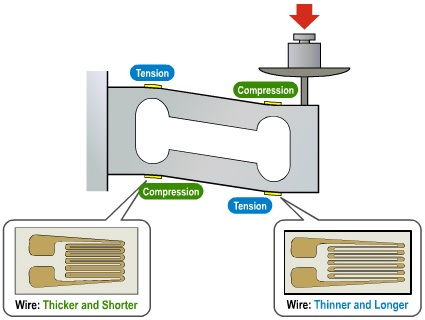
\includegraphics[height=2.8cm]{images/load_cell.jpg}
\end{center}
\caption{Schéma d'une cellule de charge avec jauge de contrainte (image : \cite{sparkfun}).}
\label{fig:load_cell_sparkfun}
\end{figure}
\end{block}
\end{frame}

\begin{frame}
\begin{block}{Comment mesurer les variations ?}
\pause
\begin{itemize}
\item Le pont Wheatstone
\pause
\begin{itemize}
\item Permet de transformer la mesure de la résistance en une mesure de tension
\pause
\item Toutefois le signal est aussi très faible (de l'ordre du $mV$)
\pause
\end{itemize}
\end{itemize}

\begin{figure}
\begin{center}
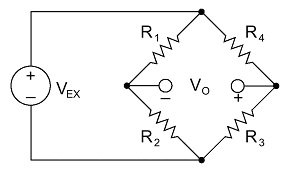
\includegraphics[height=3cm]{images/wheatstone_bridge.jpg}
\end{center}
\caption{Schéma d'un pont de Wheatstone avec $V_{EX}$ la tension d'alimentation et $V_O$ la tension de sortie (site internet de source : \cite{wheatstone}).}
\label{fig:wheatstone_bridge}
\end{figure}
\end{block}
\end{frame}

\begin{frame}
\begin{block}{Comment amplifier le signal ?}
\begin{itemize}
\item Les amplificateurs HX711
\pause
\begin{itemize}
\item Prennent un pont de wheatstone en entrée
\pause
\item On peut les connecter aux pins digitales de l'Arduino
\pause
\end{itemize}
\end{itemize}

\begin{figure}
\begin{center}
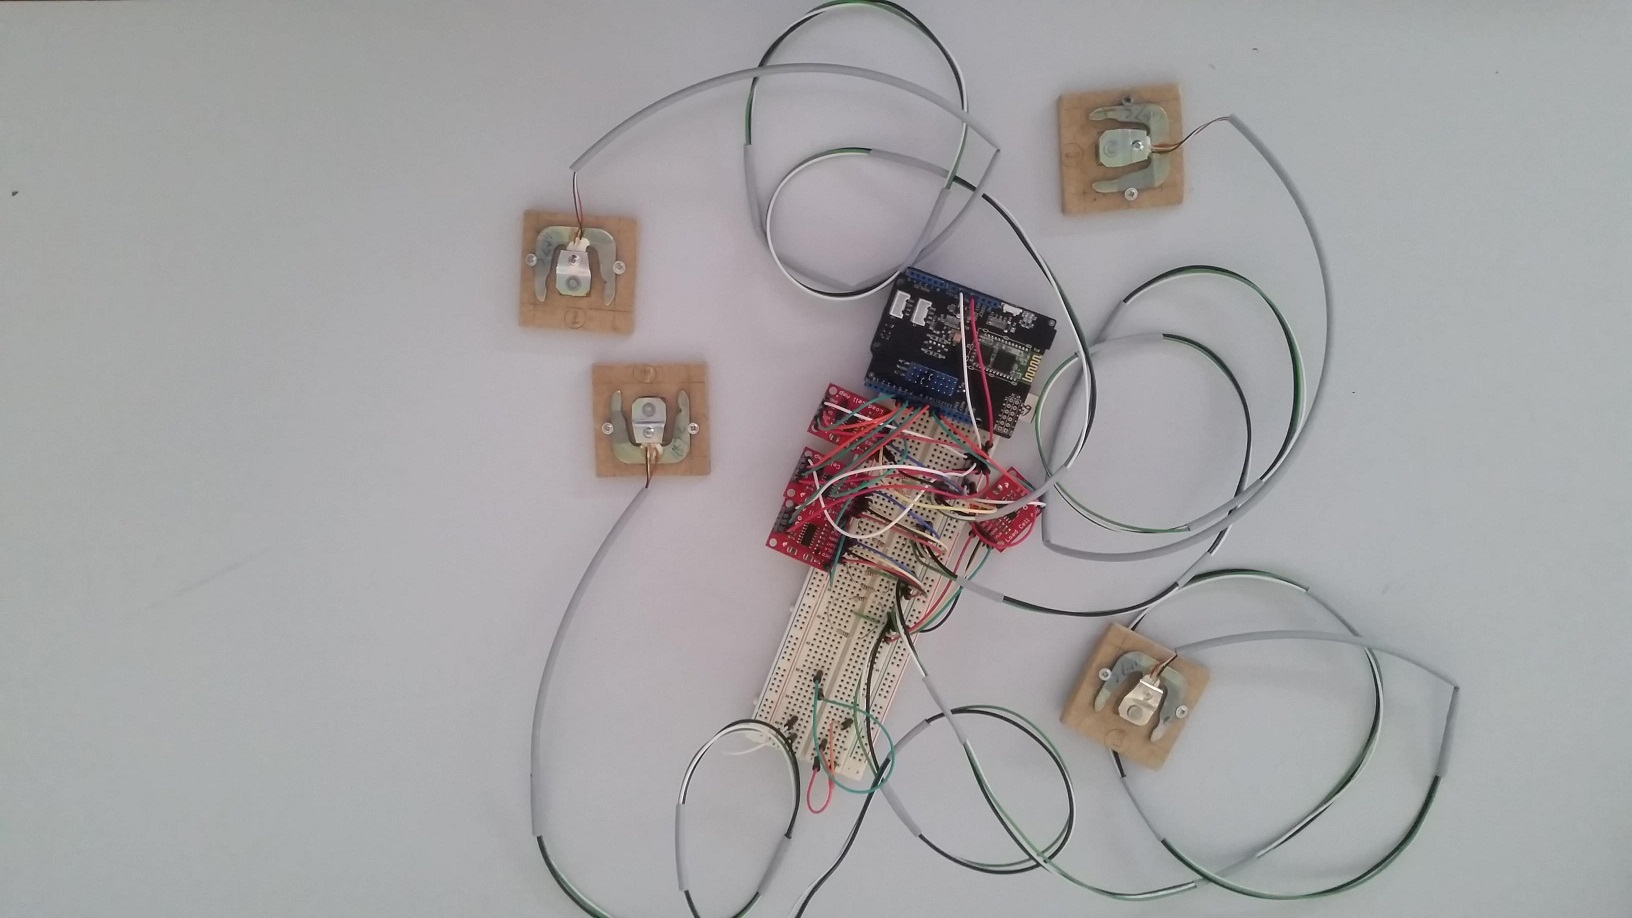
\includegraphics[height=3cm]{images/load_sensor_connected.jpg}
\end{center}
\caption{4 cellules de charges en demi-pont connectées à l'Arduino en utilisant des amplis HX711.}
\label{fig:load_sensor_connected}
\end{figure}
\end{block}
\end{frame}

\section{L'Arduino}
\begin{frame}
\begin{block}{L'Arduino}
\pause
\begin{itemize}
\item C'est un microcontrôleur
\pause
\item Peut recevoir des données analogiques ou digitales, les traiter, et les envoyer par série
\pause
\item Utilise un compilateur \texttt{avr-g++} (C/C++)
\pause
\item Peut utiliser un shield Bluetooth qui permet d'envoyer des données par Bluetooth
\end{itemize}
\end{block}
\end{frame}

\begin{frame}
\begin{block}{La programmation de l'Arduino}
\pause
\begin{itemize}
\item Le code de l'Arduino lit les données à partir des pins digitales
\pause
\item Il utilise une libraire construite pour les amplificateurs, appelée \textit{HX177} \cite{hx711}
\pause
\item Le code est aussi capable de faire une tare sur les amplificateurs
\end{itemize}
\end{block}
\end{frame}

\section{Les applications}
\begin{frame}
\begin{block}{Les applications}
\pause
\begin{itemize}
\item 2 applications diffèrentes :
\pause
\begin{itemize}
\item Application PC (Windows/OSX/Linux)
\pause
\item Application Android
\pause
\item Construites en \texttt{Java} avec \textit{Eclipse} et \textit{Android Studio}
\end{itemize}
\item Se divisent en 2 parties générales :
\pause
\begin{itemize}
\item La communication en série
\pause
\item La modélisation de la chaise et la visualisation
\end{itemize}
\end{itemize}
\end{block}
\end{frame}

\subsection{La communication en série}
\begin{frame}
\begin{block}{La communication en série}
\pause
\begin{itemize}
\item Basée sur la librairie \texttt{jSerialComm}
\pause
\item Ce module permet de :
\pause
\begin{itemize}
\item Trouver les ports sériales disponibles sur la machine
\pause
\item Se connecter aux ports et établir un flux de communication (envoyer/recevoir des données)
\pause
\item Interpréter les données d'entrée
\pause
\item Fermer le flux de communication et se déconnecter
\end{itemize}
\end{itemize}
\end{block}
\end{frame}

\subsection{La modélsation de la chaise}
\begin{frame}
\begin{block}{La modélsation de la chaise}
\pause
\begin{itemize}
\item Objet "parent" : chaise
\pause
\begin{itemize}
\item Objet "enfant" : pied
\pause
\begin{itemize}
\item Comporte un ID unique associé à l'amplificateur correspondant
\pause
\item Comporte une position
\pause
\item Comporte une valeur
\end{itemize}
\item Comporte une "zone optimale" (appelée "deadzone") :
\pause
\begin{itemize}
\item Position
\pause
\item Rayon
\pause
\end{itemize}
\item Comporte un barycentre
\end{itemize}
\end{itemize}
\end{block}
\end{frame}

\begin{frame}
\begin{block}{Comment changer de référentiel ?}
\begin{figure}[htbp]
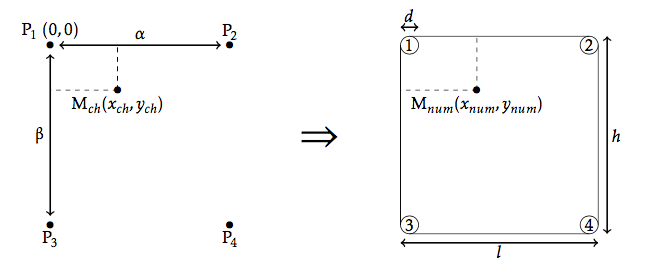
\includegraphics[height=4cm]{images/refs}
\caption{Le même point exprimé en deux référentiels : \textit{réel} (à gauche) et \textit{numérique} (à droite).}
\label{fig:visualisation_referentiels}
\end{figure}
\end{block}
\end{frame}

\begin{frame}
\begin{block}{La visualisation}
\begin{figure}[htbp]
\begin{center}

\includegraphics[height=5cm]{images/screenshot_pc1}
\end{center}
\caption{L'application PC.}
\label{fig:screenshot_pc}
\end{figure}
\end{block}
\end{frame}

\section{Conclusion}
\begin{frame}
\begin{block}{Conclusion}
\pause
\begin{itemize}
\item Avantages :
\pause
\begin{itemize}
\item Compatibilité avec plusieurs types de chaises (par exemple, une chaise à 3 pieds)
\pause
\item Facile à utiliser
\pause
\item Petite consommation électrique 
\pause
\item Compatibilité avec plusieurs plateformes (PC/mobile, Windows/OSX/Linux/Android)
\pause
\end{itemize}
\item Améliorations possibles :
\pause
\begin{itemize}
\item Fabriquer un montage qui rend l'utilisation plus facile (par exemple construire des boites en aluminium pour les cellules et une boite métallique pour l'Arduino et les amplificateurs)
\pause
\item Construire une application iOS
\pause
\item Construire un meilleur GUI
\end{itemize}
\end{itemize}
\end{block}
\end{frame}

\subsection*{Bibliographie}
\begin{frame}
\frametitle{Bibliographie}
\begin{thebibliography}{99}
{\tiny \bibitem{site-arduino} Arduino, \textit{Le site officiel d'Arduino}. 2017. \texttt{\tiny URL : https://www.arduino.cc/} (visité le 26/04/2017).

\bibitem{ntu-swing} Nanyang Technological University, \textit{Java Programming Tutorial - Custom Graphics}. 2016. \texttt{\tiny URL : http://www.ntu.edu.sg/home/ehchua/programming/java/J4b\_CustomGraphics.html} (visité le 26/04/2017).

\bibitem{load-cell} Electronics Stack Exchange, \textit{How to mount a Half Bridge Load cell}. 2016. \texttt{\tiny URL : https://electronics.stackexchange.com/questions/233574/how-to-mount-a-half-bridge-load-cell} (visité le 26/04/2017).

\bibitem{hx711} bodge, \textit{HX711 Arduino library}. 2016. \texttt{\tiny URL : https://github.com/bogde/HX711} (visité le 26/04/2017).

\bibitem{android-studio} Google, \textit{Android Studio}. 2017. \texttt{\tiny URL : https://developer.android.com/studio/index.html} (visité le 26/04/2017).

\bibitem{repo-github} KOKKONIS Dimitrios, LOCHE Jérémy, \textit{pression}. 2017. \texttt{\tiny URL : https://github.com/kokkonisd/pression} (visité le 26/04/2017).

\bibitem{sparkfun} Sparkfun, \textit{Getting Started with Load Cells}. 2016. \texttt{\tiny URL : https://learn.sparkfun.com/tutorials/getting-started-with-load-cells} (visité le 26/04/2017).

\bibitem{wheatstone} National Instruments, \textit{Comment effectuer une mesure avec une cellule de charge ou un transducteur de pression}. 2013. \texttt{\tiny URL : http://www.ni.com/tutorial/7138/fr/} (visité le 26/04/2017).}
\end{thebibliography}
\end{frame}

\subsection*{Liens utiles}
\begin{frame}
\frametitle{Liens utiles}
\begin{itemize}
\item \url{www.polytech.univ-tours.fr}
\end{itemize}
\end{frame}

\end{document}
